\documentclass[../notes.tex]{subfiles}

\pagestyle{main}
\renewcommand{\chaptermark}[1]{\markboth{\chaptername\ \thechapter\ (#1)}{}}
\setcounter{chapter}{12}

\begin{document}




\chapter{Dynamical Systems and Chaos}
\section{Introduction to Dynamical Systems; Phase Portraits}
\begin{itemize}
    \item \marginnote{11/27:}\textbf{Dyanmical system}: A system of first-order ODEs.
    \item Example: Flows on a line.
    \begin{figure}[h!]
        \centering
        \begin{tikzpicture}
            \footnotesize
            \draw [
                -stealth,
                decoration={
                    markings,
                    mark=at position 0.15 with \arrow{<},
                    mark=at position 0.40 with \arrow{>},
                    mark=at position 0.65 with \arrow{>},
                    mark=at position 0.87 with \arrow{<}
                },
                postaction=decorate
            ] (-1,0) -- (1,0) node[right]{$x$};
            \draw [-stealth] (0,-0.5) -- (0,1.5) node[above]{$f(x)=\dot{x}$};
    
            \draw [grx,thick,<->] plot[domain=-0.6:0.6] (\x,{1-4*\x*\x});
    
            \filldraw [fill=white] (-0.5,0) circle (1pt);
            \filldraw              (0.5,0)  circle (1pt);
        \end{tikzpicture}
        \caption{Dynamical flows on a line.}
        \label{fig:flowsLine}
    \end{figure}
    \begin{itemize}
        \item Consider
        \begin{equation*}
            \dot{x} = -x^2+4
        \end{equation*}
        \item Graph $f(x)=\dot{x}$, as above.
        \item When the graph is negative, a particle on the line heads to the left; when it is positive, the particle heads to the right. We indicate this with arrows.
        \item Then we indicate \textbf{fixed points} with circles, \textbf{unstable} ones with unfilled circles and \textbf{stable} ones with filled circles.
        \item How do we determine fixed points and stability mathematically?
        \item Fixed points: Solving $\dot{x}=0$ yields $x^*=\pm 2$ as fixed points.
        \item Stability: Consider a point a small distance away from $x^*$ at $x=x^*+\xi$.
        \begin{itemize}
            \item Approximate $\dot{x}$ near $x^*$ via
            \begin{equation*}
                \dot{x} = f(x) = f(x^*+\xi) \approx f(x^*)+\eval{\pdv{f}{x}}_{x^*}\xi+O(\xi^2)
            \end{equation*}
            \item Then since $f(x^*)=0$ and we neglect $O(\xi^2)$ for small $\xi$, we have that
            \begin{equation*}
                \dot{x} = \dot{\xi} = \eval{\pdv{f}{x}}_{x^*}\xi
            \end{equation*}
            \item Looking at Figure \ref{fig:flowsLine}, we can see that the fixed point is stable if $\eval{\pdv*{f}{x}}_{x^*}\xi<0$ and unstable if $\eval{\pdv*{f}{x}}_{x^*}\xi>0$.
        \end{itemize}
    \end{itemize}
    \item \textbf{Fixed point}: A point at which $\dot{x}=0$.
    \item \textbf{Unstable} (fixed point): A fixed point with the flow heading away from it.
    \item\textbf{Stable} (fixed point): A fixed point with the flow heading toward it.
    \item Let's promote ourselves up a dimension to the 2D phase plane.
    \item Example: Pendulum.
    \begin{figure}[h!]
        \centering
        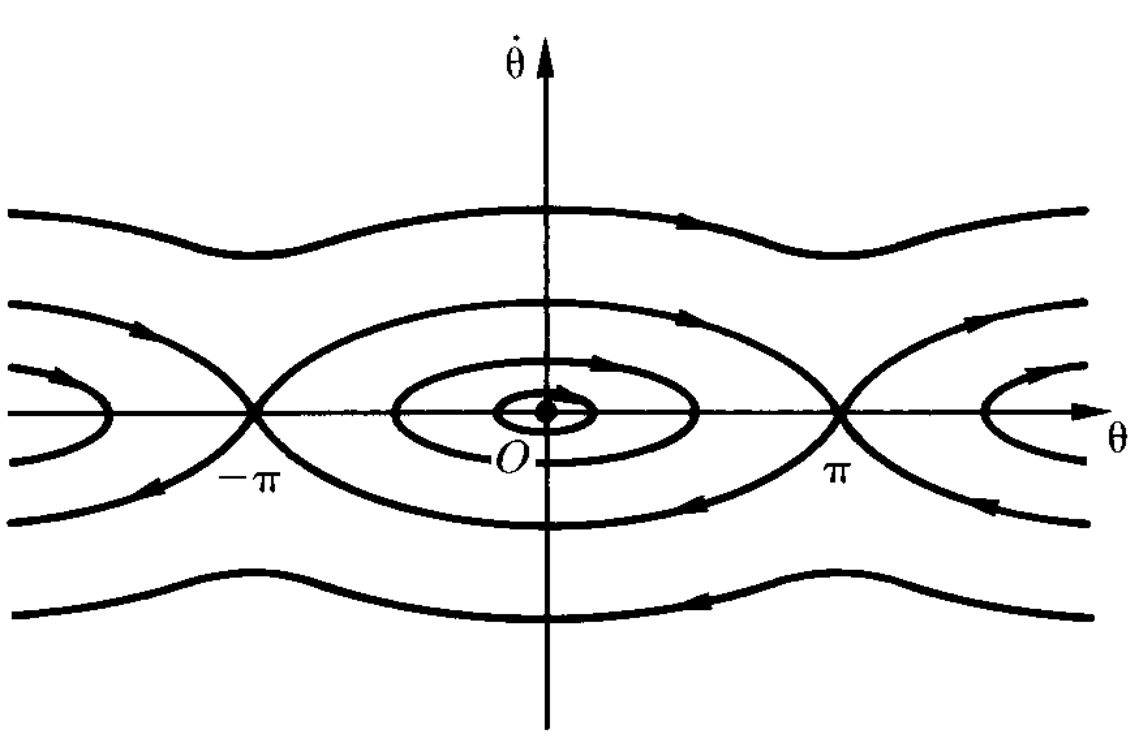
\includegraphics[width=0.4\linewidth]{../ExtFiles/flowsPendulum.png}
        \caption{Dynamical flows of a pendulum.}
        \label{fig:flowsPendulum}
    \end{figure}
    \begin{itemize}
        \item Recall that the Hamiltonian for such a system is
        \begin{equation*}
            H = \frac{p_\theta^2}{2m\ell^2}-mg\ell\cos\theta
        \end{equation*}
        \item Thus, Hamilton's equations are
        \begin{align*}
            -\dot{p}_\theta &= \pdv{H}{\theta} = mg\ell\sin\theta&
            \dot{\theta} &= \pdv{H}{p_\theta} = \frac{p_\theta}{m\ell^2}
        \end{align*}
        \item This gives us a system of first-order ODEs.
        \item Fixed points: $\dot{\theta}=0$ implies $p_\theta=0$, implies $\dot{p}_\theta=0$, implies $\sin\theta=0$ implies $\theta=0,\pm\pi,\dots$.
        \item We may now draw a \textbf{phase portrait}.
        \item We get circles corresponding to the switch between momentum and potential energy.
        \item At the fixed points, we have a special \textbf{separatrix}; the particle takes an infinite amount of time to get to the fixed point with unstable equilibrium.
        \item Then the paths at the top and bottom are other trajectories corresponding to swinging all the way around in one direction or another.
        \item It is traditional to call these paths \emph{trajectories}, even though they are not physical trajectories $x(t)$.
    \end{itemize}
    \item \textbf{Phase portrait}: A plot that gives the paths of particles at all times.
    \begin{itemize}
        \item What you gain from a phase portrait is all of the paths, but what you lose is all of the dynamical information (i.e., you have no idea how fast anything is going).
    \end{itemize}
    \item Linear stability in 2D.
    \begin{itemize}
        \item In general, we have a system of two first-order ODEs as follows.
        \begin{equation*}
            \begin{cases}
                \dot{x} = f(x,y)\\
                \dot{y} = g(x,y)
            \end{cases}
        \end{equation*}
        \item Let $(x^*,y^*)$ be a fixed point.
        \item Then, Taylor expanding, we get
        \begin{align*}
            \dot{x} &= f(x^*+\xi,y^*+\eta) \approx f(x^*,y^*)+\eval{\pdv{f}{x}}_{x^*,y^*}\xi+\eval{\pdv{f}{y}}_{x^*,y^*}\eta+O(\xi^2,\eta^2)\\
            \dot{y} &= g(x^*+\xi,y^*+\eta) \approx g(x^*,y^*)+\eval{\pdv{g}{x}}_{x^*,y^*}\xi+\eval{\pdv{g}{y}}_{x^*,y^*}\eta+O(\xi^2,\eta^2)
        \end{align*}
        \item From here, we obtain a matrix of coefficients called the \textbf{Jacobian matrix}, $J$, as follows.
        \begin{equation*}
            \begin{pmatrix}
                \dot{x}\\
                \dot{y}\\
            \end{pmatrix}
            =
            \begin{pmatrix}
                \dot{\xi}\\
                \dot{\eta}\\
            \end{pmatrix}
            =
            \begin{pNiceMatrix}
                \pdv{f}{x} & \pdv{f}{y}\\
                \pdv{g}{x} & \pdv{g}{y}\\
            \end{pNiceMatrix}
            \begin{pmatrix}
                \xi\\
                \eta\\
            \end{pmatrix}
        \end{equation*}
        \begin{itemize}
            \item The directions of exponential growth and decay occur in the eigendirections of the Jacobian matrix!
        \end{itemize}
        \item Indeed, in these 2D systems, we can classify the fixed point based on the eigenvalues of $J$.
        \item Solve for the eigenvalues using the following formula.
        \begin{equation*}
            \lambda_{1,2} = \frac{1}{2}\left[ \tr(J)\pm\sqrt{\tr(J)^2-4\det(J)} \right]
        \end{equation*}
        \item For stability, we need the real parts of both eigenvalues to be less than zero.
    \end{itemize}
    \item There are three important classifications of such systems.
    \begin{figure}[h!]
        \centering
        \begin{subfigure}[b]{0.24\linewidth}
            \centering
            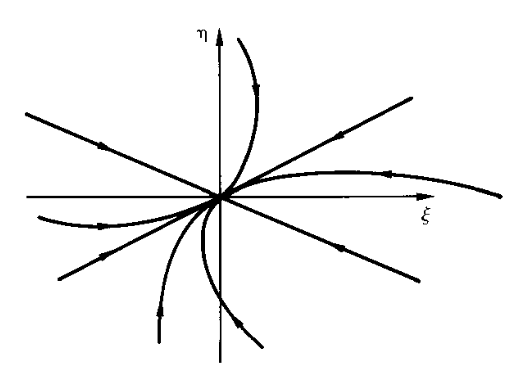
\includegraphics[width=0.95\linewidth]{../ExtFiles/classifyFixedPointsa.png}
            \caption{Node.}
            \label{fig:classifyFixedPointa}
        \end{subfigure}
        \begin{subfigure}[b]{0.24\linewidth}
            \centering
            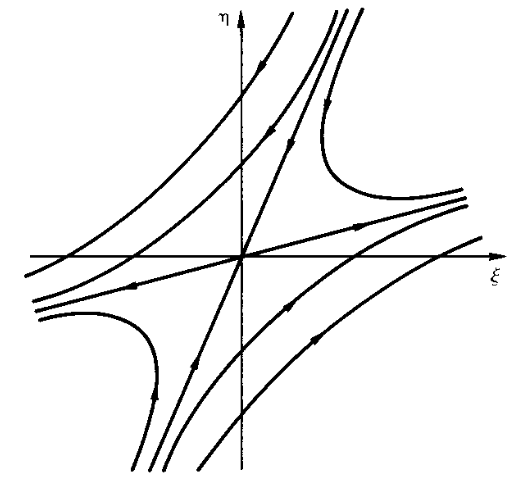
\includegraphics[width=0.95\linewidth]{../ExtFiles/classifyFixedPointsb.png}
            \caption{Saddle.}
            \label{fig:classifyFixedPointb}
        \end{subfigure}
        \begin{subfigure}[b]{0.24\linewidth}
            \centering
            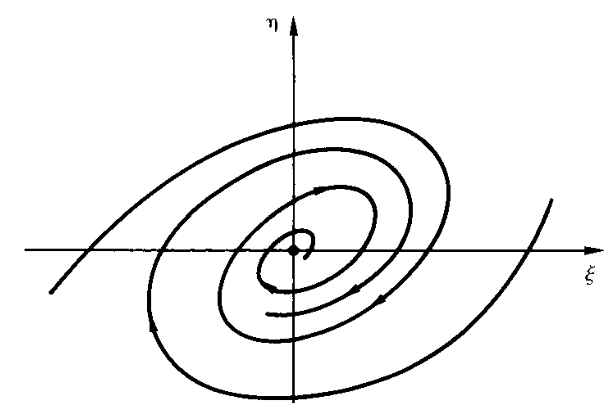
\includegraphics[width=0.95\linewidth]{../ExtFiles/classifyFixedPointsc.png}
            \caption{Spiral.}
            \label{fig:classifyFixedPointc}
        \end{subfigure}
        \begin{subfigure}[b]{0.24\linewidth}
            \centering
            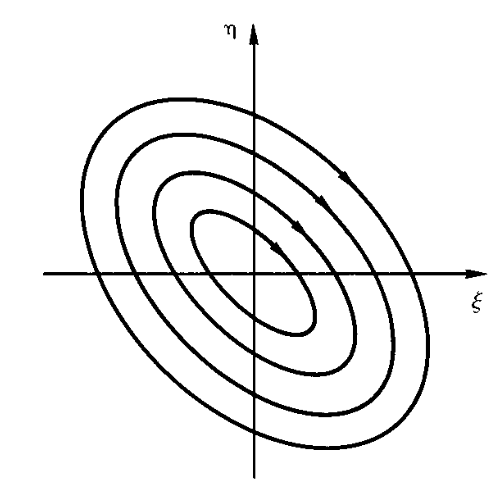
\includegraphics[width=0.95\linewidth]{../ExtFiles/classifyFixedPointsd.png}
            \caption{Center.}
            \label{fig:classifyFixedPointd}
        \end{subfigure}
        \caption{Classifying fixed points.}
        \label{fig:classifyFixedPoint}
    \end{figure}
    \begin{enumerate}
        \item \textbf{Nodes} happen when both $\lambda_1,\lambda_2$ are real and both are positive \emph{or} both are negative.
        \begin{itemize}
            \item Everything falls into the fixed point in the case $\lambda_1,\lambda_2<0$; some things directly (along eigendirections) and other things along curved paths.
            \item Alternatively, if $\lambda_1,\lambda_2>0$, then everything gets blown away.
        \end{itemize}
        \item If one is greater than zero and one is less than zero, we get a \textbf{saddle} point.
        \item If there are some imaginary parts, we get circulation and spiraling. From the eigenvalue formula, we can see that $\lambda_1,\lambda_2=a\pm bi$ are complex conjugates.
        \begin{itemize}
            \item If real parts are negative, we spiral inwards; if positive, we spiral outwards.
            \item There's also the concept of a \textbf{center}; when $\lambda_1,\lambda_2$ are purely imaginary, we get pure circulation where things choose their orbit and stay on it. This is also \emph{stable}, even though things don't fall into the node.
        \end{itemize}
    \end{enumerate}
    \item A handy picture to help us classify any fixed point we want in two dimensions.
    \begin{figure}[h!]
        \centering
        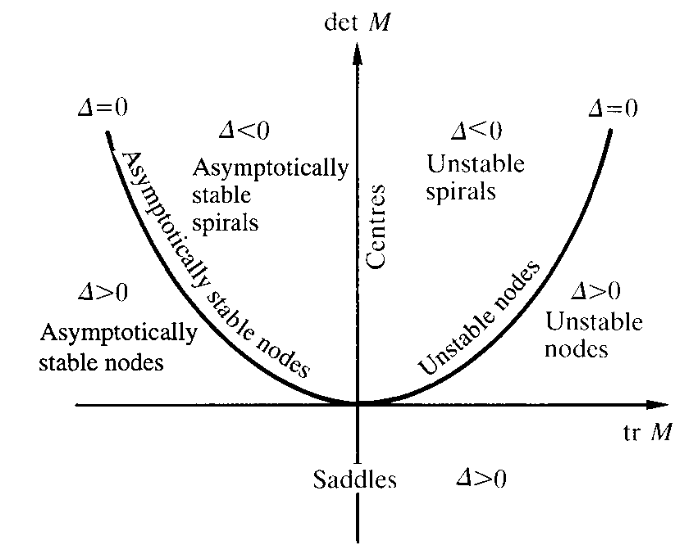
\includegraphics[width=0.4\linewidth]{../ExtFiles/fixedPointParabola.png}
        \caption{Fixed points parabola.}
        \label{fig:fixedPointParabola}
    \end{figure}
    \begin{itemize}
        \item If we look at systems defined in terms of their trace and determinant, there is a sideways parabola defined by the discriminant of the eigenvalue formula, i.e., via $\tr(J)^2-4\det(J)=0$.
        \item Various paths live in different parts of the map.
    \end{itemize}
\end{itemize}




\end{document}